\lstset{language=[Sharp]C}
\chapter{Allgemeines}
\textit{Shulker-Connect} ist die Softwarelösung, um von externen Ressourcen aus mit dem Türschloss zu kommunizieren.

Dies haben wir mittels eines ASP.NET Core Web API Servers umgesetzt. Dieser Server stellt eine REST-API zur Verfügung, 
auf die von beliebigen Applikationen aus zugegriffen werden kann, um Shulker-Core Befehle mitzuteilen und Abfragen zu stellen.

In der Shulker-Zutrittsmanagement-Lösung wird der Shulker-Connect API-Server von Shulker-Mobile verwendet. 
Durch die Implementierung von Shulker-Connect könnten allerdings auch beliebige andere Applikationen, 
wie z.B.: eine Steuerungs-Website, das Türschloss steuern. 
So könnten später auf einfacher weise die Steuerungsmöglichkeiten des Schlosses erweitert werden.

\section{Verbindung zu Shulker-Core}
\textit{Shulker-Connect} muss mit \textit{Shulker-Core} kommunizieren, sodass eine API-Anfrage an Shulker-Connect tatsächlich
auch das Türschloss steuern kann.
Dies kann über \textit{inter process communication sockets} erreicht werden. 
Um eine stabile und effiziente Kommunikation mit der auf dem Raspberry PI laufenden Rust-Software Shulker-Core zu 
gewährleisten, haben wir auf beiden Endpunkten \textit{POSIX-Sockets} implementiert.

Beim Start von Shulker-Connect werden zwei neue Threads erstellt: Ein Listener-Thread und ein Sender-Thread.
Beide Threads erstellen ein \textit{socket}-Objekt, das auf eine Verbindung von \textit{Shulker-Core} wartet.
Wird diese hergestellt, sind die Threads bereit, Daten zu senden bzw. zu empfangen.
In Shulker werden alle Nachrichten im \textit{UTF8}-Format gesendet.

\subsection{Was sind POSIX-Sockets?}
\textit{POSIX local inter-process communication sockets} (auch Unix Domain Sockets oder IPC Sockets genannt) ermöglichen
eine bidirektionale Kommunikationsverbindung für die Interprozesskommunikation (IPC) auf UNIX basierenden Systemen.
Hierbei wird von beiden Kommunikations-Partnern eine Datei vereinbart, über diese die Kommunikation erfolgt. \cite{ipcsockets}
Die Kommunikation zwischen Shulker-Connect und Shulker-Core muss nicht verschlüsselt werden, da eine Kompromittierung des
Raspberry-Pi's die einzige Möglichkeit darstellt, diese Kommunikation mitzulesen, da sie komplett lokal abläuft. 

\subsection{Aufbau der POSIX-Nachrichten}
Da Shulker-Connect und Shulker-Core über String-Nachrichten miteinander kommunizieren, haben wir einen
Format festgelegt, an welchen sich alle Nachrichten der Kommunikation halten müssen.


Alle gesendeten Nachrichten werden im JSON-Format gesendet. Jede Nachricht beinhaltet immer ein Attribut namens
\textit{"method"}, dieses ist der Identifikator der Anfrage und lässt sich mit Routen von Web-Diensten vergleichen.
Zusätzlich können beliebige andere Attribute, die für die jeweilige Route relevant sind, in der Nachricht mitgesendet werden.

\subsubsection{Beispiel}
Shulker-Connect sendet folgenden String an Shulker-Core.
\begin{lstlisting}
{"method":"GetPins"}
\end{lstlisting}
Shulker-Core erhält die Nachricht, und schaut sich die \textit{method} des JSON-Strings an.
Die method \textit{GetPins} definiert, dass Shulker-Connect eine Liste alle Pins anfordert.

Shulker-Core sendet nun Beispielhaft folgende Nachricht an Shulker-Connect zurück.
\begin{lstlisting}
{
    "method":"PinList",
    "pins":[
        {
            "label":"Oma",
            "uuid":"7cb46a16-9794-486c-89b5-997b32f9b81c",
            "start_time":"2022-03-19T16:40:34.098Z",
            "end_time":"2022-05-01T15:00:00Z",
            "uses_left":-1
        }
    ]
    }
\end{lstlisting}
Somit kann Shulker-Connect anhand der method \textit{PinList} erkennen, dass es sich bei dieser Nachricht um die Liste
aller Pins, also einer Antwort der vorherigen Anfrage, haltet.

\section{Verschlüsselung der Anfragen von Shulker-Mobile zum API-Server}
Da es sich bei einem Haustürschloss um eine sehr wichtige und sichere Vorrichtung handelt, muss natürlich auch die
Kommunikation zu diesem auf sicherem Wege erfolgen. Das Türschloss soll schließlich mittels App von der ganzen Welt
aus steuerbar sein.

Um dieses Problem zu lösen und eine definitiv sichere und verschlüsselte Kommunikation zu gewährleisten, haben wir uns dazu 
entschieden, den Nutzer zu zwingen, einen VPN-Tunnel zum lokalen Netzwerk, in dem auch das Türschloss steht, herstellen
zu müssen, falls dieser sich nicht im lokalen Netzwerk befindet. So sicher wie das VPN-Protokoll, dass zur Verbindung genützt
wird ist, ist somit auch die Verbindung zum Türschloss.

Als zusätzlichen Vorteil bietet diese Lösung auch, dass das Türschloss nicht vom öffentlichen Internet aus erreichbar sein muss.
Dies sichert das Gesamtsystem noch einmal zusätzlich ab und schließt einen wichtigen Angriffsvektor.

\section{Authentifizierung am Server}
Immer dann, wenn Shulker-Mobile auf Routen von Shulker-Connect zugreifen möchte, muss sich der Client Authentifizieren.
Diese Authentifizierung haben wir mittels eines Session-Systems umgesetzt.

Um dies am Server umzusetzen, haben wir eine \textit{SessionManager}-Klasse programmiert. Diese Klasse folgt dem
\textit{Singleton Pattern} und verwaltet alle aktiven Sessions. In Shulker bleibt eine Session 20 Minuten valide, dann
muss eine neue generiert werden.

Der Session-String selbst setzt sich aus 32 kryptografisch zufällig ausgewählten Buchstaben bzw. Zahlen zusammen.

\section{Beispielhafter Ablauf einer Anfrage zu Shulker-Connect}
Um zu demonstrieren, wie der Ablauf einer Anfrage an Shulker-Connect intern gehandhabt wird, schauen wir uns das Generieren
eines Session-Tokens an.

\begin{figure}[H]
    \begin{center}
        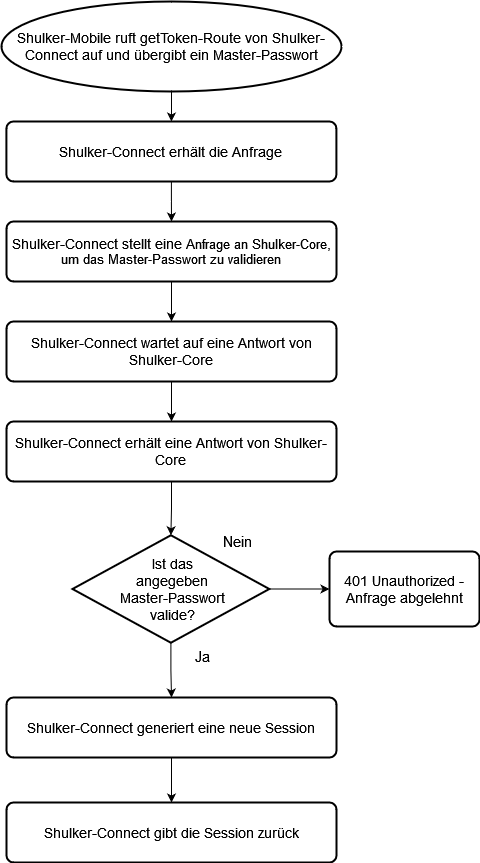
\includegraphics[width=.6\textwidth]{images/connect/AblaufGetToken.png}
        \caption{Ablauf der Abfrage zum generieren einer neuen Session}
    \end{center}
\end{figure}

Als erstes ruft Shulker-Mobile beim Start der App die Route \textit{/api/Session/getToken/{secret}} auf.
Diese Route nimmt einen Parameter namens \textit{secret} - das ist das Master-Passwort des Türschlosses.

Shulker-Connect nimmt die Anfrage in der \textit{getToken} Methode innerhalb des \textit{Session Controllers} entgegen, 
wie der Namen des Controllers verdeutlicht, handhabt dieser die Sessions.

Im Anschluss stellt Shulker-Connect über den \textit{POSIX-Socket} in Richtung Shulker-Core eine Anfrage, um zu
überprüfen, ob das Master-Passwort Valide ist. Genaueres zum Aufbau der Anfragen folgt später.
Shulker-Connect wartet währenddessen asynchron auf die Antwort von Shulker-Core.

Sobald eine Antwort von Shulker-Core über den POSIX-Socket empfangen wurde, läuft die \textit{getToken} 
Methode weiter. Dort wird anschließend, abhängig davon ob das angegebene Master-Passwort valide ist, eine neue Session 
erstellt und zurückgegeben, oder die Anfrage über den HTTP-Error \textit{401 Unauthorized} abgelehnt.